\documentclass[twoside]{book}

% Packages required by doxygen
\usepackage{fixltx2e}
\usepackage{calc}
\usepackage{doxygen}
\usepackage[export]{adjustbox} % also loads graphicx
\usepackage{graphicx}
\usepackage[utf8]{inputenc}
\usepackage{makeidx}
\usepackage{multicol}
\usepackage{multirow}
\PassOptionsToPackage{warn}{textcomp}
\usepackage{textcomp}
\usepackage[nointegrals]{wasysym}
\usepackage[table]{xcolor}

% NLS support packages
\usepackage[brazil]{babel}
% Font selection
\usepackage[T1]{fontenc}
\usepackage[scaled=.90]{helvet}
\usepackage{courier}
\usepackage{amssymb}
\usepackage{sectsty}
\renewcommand{\familydefault}{\sfdefault}
\allsectionsfont{%
  \fontseries{bc}\selectfont%
  \color{darkgray}%
}
\renewcommand{\DoxyLabelFont}{%
  \fontseries{bc}\selectfont%
  \color{darkgray}%
}
\newcommand{\+}{\discretionary{\mbox{\scriptsize$\hookleftarrow$}}{}{}}

% Page & text layout
\usepackage{geometry}
\geometry{%
  a4paper,%
  top=2.5cm,%
  bottom=2.5cm,%
  left=2.5cm,%
  right=2.5cm%
}
\tolerance=750
\hfuzz=15pt
\hbadness=750
\setlength{\emergencystretch}{15pt}
\setlength{\parindent}{0cm}
\setlength{\parskip}{3ex plus 2ex minus 2ex}
\makeatletter
\renewcommand{\paragraph}{%
  \@startsection{paragraph}{4}{0ex}{-1.0ex}{1.0ex}{%
    \normalfont\normalsize\bfseries\SS@parafont%
  }%
}
\renewcommand{\subparagraph}{%
  \@startsection{subparagraph}{5}{0ex}{-1.0ex}{1.0ex}{%
    \normalfont\normalsize\bfseries\SS@subparafont%
  }%
}
\makeatother

% Headers & footers
\usepackage{fancyhdr}
\pagestyle{fancyplain}
\fancyhead[LE]{\fancyplain{}{\bfseries\thepage}}
\fancyhead[CE]{\fancyplain{}{}}
\fancyhead[RE]{\fancyplain{}{\bfseries\leftmark}}
\fancyhead[LO]{\fancyplain{}{\bfseries\rightmark}}
\fancyhead[CO]{\fancyplain{}{}}
\fancyhead[RO]{\fancyplain{}{\bfseries\thepage}}
\fancyfoot[LE]{\fancyplain{}{}}
\fancyfoot[CE]{\fancyplain{}{}}
\fancyfoot[RE]{\fancyplain{}{\bfseries\scriptsize Gerado por Doxygen }}
\fancyfoot[LO]{\fancyplain{}{\bfseries\scriptsize Gerado por Doxygen }}
\fancyfoot[CO]{\fancyplain{}{}}
\fancyfoot[RO]{\fancyplain{}{}}
\renewcommand{\footrulewidth}{0.4pt}
\renewcommand{\chaptermark}[1]{%
  \markboth{#1}{}%
}
\renewcommand{\sectionmark}[1]{%
  \markright{\thesection\ #1}%
}

% Indices & bibliography
\usepackage{natbib}
\usepackage[titles]{tocloft}
\setcounter{tocdepth}{3}
\setcounter{secnumdepth}{5}
\makeindex

% Hyperlinks (required, but should be loaded last)
\usepackage{ifpdf}
\ifpdf
  \usepackage[pdftex,pagebackref=true]{hyperref}
\else
  \usepackage[ps2pdf,pagebackref=true]{hyperref}
\fi
\hypersetup{%
  colorlinks=true,%
  linkcolor=blue,%
  citecolor=blue,%
  unicode%
}

% Custom commands
\newcommand{\clearemptydoublepage}{%
  \newpage{\pagestyle{empty}\cleardoublepage}%
}

\usepackage{caption}
\captionsetup{labelsep=space,justification=centering,font={bf},singlelinecheck=off,skip=4pt,position=top}

%===== C O N T E N T S =====

\begin{document}

% Titlepage & ToC
\hypersetup{pageanchor=false,
             bookmarksnumbered=true,
             pdfencoding=unicode
            }
\pagenumbering{roman}
\begin{titlepage}
\vspace*{7cm}
\begin{center}%
{\Large Projeto\+LP \\[1ex]\large 01 }\\
\vspace*{1cm}
{\large Gerado por Doxygen 1.8.11}\\
\end{center}
\end{titlepage}
\clearemptydoublepage
\tableofcontents
\clearemptydoublepage
\pagenumbering{arabic}
\hypersetup{pageanchor=true}

%--- Begin generated contents ---
\chapter{Índice dos Arquivos}
\section{Lista de Arquivos}
Esta é a lista de todos os arquivos documentados e suas respectivas descrições\+:\begin{DoxyCompactList}
\item\contentsline{section}{include/{\bfseries file\+Handler.\+h} }{\pageref{fileHandler_8h}}{}
\item\contentsline{section}{include/{\bfseries matriz.\+h} }{\pageref{matriz_8h}}{}
\item\contentsline{section}{include/{\bfseries mem\+Manager.\+h} }{\pageref{memManager_8h}}{}
\item\contentsline{section}{src/\hyperlink{matriz_8cpp}{matriz.\+cpp} \\*Programa que faz multiplicações de matrizes e gera estatísticas sobre o tempo de execução  Rodrigo Rocha Moriyama \href{mailto:rodrigo.oi@hotmail.com}{\tt rodrigo.\+oi@hotmail.\+com} \&\& Ariel de Oliveira Corrêa \href{mailto:ariel.oliveira01@gmail.com}{\tt ariel.\+oliveira01@gmail.\+com} }{\pageref{matriz_8cpp}}{}
\item\contentsline{section}{src/\hyperlink{memManager_8cpp}{mem\+Manager.\+cpp} \\*Funções que alocam e desalocam espaços da memória utilizados pelas matrizes  Rodrigo Rocha Moriyama \href{mailto:rodrigo.oi@hotmail.com}{\tt rodrigo.\+oi@hotmail.\+com} \&\& Ariel de Oliveira Corrêa \href{mailto:ariel.oliveira01@gmail.com}{\tt ariel.\+oliveira01@gmail.\+com} }{\pageref{memManager_8cpp}}{}
\end{DoxyCompactList}

\chapter{Arquivos}
\hypertarget{matriz_8cpp}{}\section{Referência do Arquivo src/matriz.cpp}
\label{matriz_8cpp}\index{src/matriz.\+cpp@{src/matriz.\+cpp}}


Programa que faz multiplicações de matrizes e gera estatísticas sobre o tempo de execução  Rodrigo Rocha Moriyama \href{mailto:rodrigo.oi@hotmail.com}{\tt rodrigo.\+oi@hotmail.\+com} \&\& Ariel de Oliveira Corrêa \href{mailto:ariel.oliveira01@gmail.com}{\tt ariel.\+oliveira01@gmail.\+com}  


{\ttfamily \#include \char`\"{}matriz.\+h\char`\"{}}\\*
{\ttfamily \#include $<$iostream$>$}\\*
Gráfico de dependência de inclusões para matriz.\+cpp\+:
\nopagebreak
\begin{figure}[H]
\begin{center}
\leavevmode
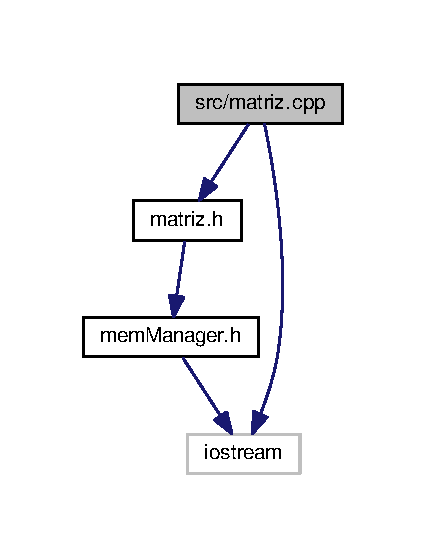
\includegraphics[width=205pt]{matriz_8cpp__incl}
\end{center}
\end{figure}
\subsection*{Funções}
\begin{DoxyCompactItemize}
\item 
{\footnotesize template$<$typename T $>$ }\\T $\ast$$\ast$ \hyperlink{matriz_8cpp_a029b21745688cbd0dedab53ac5502aba}{SomaM} (T $\ast$$\ast$M1, T $\ast$$\ast$M2, int n)
\begin{DoxyCompactList}\small\item\em Soma de duas matrizes. \end{DoxyCompactList}\item 
{\footnotesize template$<$typename T $>$ }\\T $\ast$$\ast$ \hyperlink{matriz_8cpp_a9f299c09117aa38830540e142fd7ddd1}{Mult\+MatrizesI} (T $\ast$$\ast$M1, T $\ast$$\ast$M2, int m)
\begin{DoxyCompactList}\small\item\em Multiplicação interativa das matrizes. \end{DoxyCompactList}\item 
template int $\ast$$\ast$ {\bfseries Mult\+Matrizes\+I$<$ int $>$} (int $\ast$$\ast$M1, int $\ast$$\ast$M2, int m)\hypertarget{matriz_8cpp_a1021515d786f22ce29385a32991ab922}{}\label{matriz_8cpp_a1021515d786f22ce29385a32991ab922}

\item 
{\footnotesize template$<$typename T $>$ }\\T $\ast$$\ast$ \hyperlink{matriz_8cpp_a94f514204154053dfea35221cf8819a3}{Unir\+Matriz} (T $\ast$$\ast$M, T $\ast$$\ast$M1, T $\ast$$\ast$M2, T $\ast$$\ast$M3, T $\ast$$\ast$M4, int n)
\begin{DoxyCompactList}\small\item\em União das submatrizes em uma única matriz. \end{DoxyCompactList}\item 
{\footnotesize template$<$typename T $>$ }\\void \hyperlink{matriz_8cpp_a2c80459ce9105a84612fea4a5072193b}{Atribuir\+SubM} (T $\ast$$\ast$M, T $\ast$$\ast$M1, T $\ast$$\ast$M2, T $\ast$$\ast$M3, T $\ast$$\ast$M4, int n)
\begin{DoxyCompactList}\small\item\em Atribui valores as submatrizes da função recursiva. \end{DoxyCompactList}\item 
{\footnotesize template$<$typename T $>$ }\\T $\ast$$\ast$ \hyperlink{matriz_8cpp_ab97fd7fa09ee41bcdcc03544fd61af05}{Mult\+MatrizesR} (T $\ast$$\ast$M1, T $\ast$$\ast$M2, T $\ast$$\ast$M3, int n)
\item 
template int $\ast$$\ast$ {\bfseries Mult\+Matrizes\+R$<$ int $>$} (int $\ast$$\ast$M1, int $\ast$$\ast$M2, int $\ast$$\ast$M3, int n)\hypertarget{matriz_8cpp_a597872fddb527b6c3d3ec2efbea62b8e}{}\label{matriz_8cpp_a597872fddb527b6c3d3ec2efbea62b8e}

\end{DoxyCompactItemize}


\subsection{Descrição Detalhada}
Programa que faz multiplicações de matrizes e gera estatísticas sobre o tempo de execução  Rodrigo Rocha Moriyama \href{mailto:rodrigo.oi@hotmail.com}{\tt rodrigo.\+oi@hotmail.\+com} \&\& Ariel de Oliveira Corrêa \href{mailto:ariel.oliveira01@gmail.com}{\tt ariel.\+oliveira01@gmail.\+com} 

Funções interativas e recursivas para a multiplicação das matrizes  Rodrigo Rocha Moriyama \href{mailto:rodrigo.oi@hotmail.com}{\tt rodrigo.\+oi@hotmail.\+com} \&\& Ariel de Oliveira Corrêa \href{mailto:ariel.oliveira01@gmail.com}{\tt ariel.\+oliveira01@gmail.\+com}

\begin{DoxySince}{Desde}
28/04/2017  01/05/2017 
\end{DoxySince}


\subsection{Funções}
\index{matriz.\+cpp@{matriz.\+cpp}!Atribuir\+SubM@{Atribuir\+SubM}}
\index{Atribuir\+SubM@{Atribuir\+SubM}!matriz.\+cpp@{matriz.\+cpp}}
\subsubsection[{\texorpdfstring{Atribuir\+Sub\+M(\+T $\ast$$\ast$\+M, T $\ast$$\ast$\+M1, T $\ast$$\ast$\+M2, T $\ast$$\ast$\+M3, T $\ast$$\ast$\+M4, int n)}{AtribuirSubM(T **M, T **M1, T **M2, T **M3, T **M4, int n)}}]{\setlength{\rightskip}{0pt plus 5cm}template$<$typename T $>$ void Atribuir\+SubM (
\begin{DoxyParamCaption}
\item[{T $\ast$$\ast$}]{M, }
\item[{T $\ast$$\ast$}]{M1, }
\item[{T $\ast$$\ast$}]{M2, }
\item[{T $\ast$$\ast$}]{M3, }
\item[{T $\ast$$\ast$}]{M4, }
\item[{int}]{n}
\end{DoxyParamCaption}
)}\hypertarget{matriz_8cpp_a2c80459ce9105a84612fea4a5072193b}{}\label{matriz_8cpp_a2c80459ce9105a84612fea4a5072193b}


Atribui valores as submatrizes da função recursiva. 


\begin{DoxyParams}{Parâmetros}
{\em M} & Matriz que possui os valores para as submatrizes \\
\hline
{\em M1} & Submatriz de entrada \\
\hline
{\em M2} & Submatriz de entrada \\
\hline
{\em M3} & Submatriz de entrada \\
\hline
{\em M4} & Submatriz de entrada \\
\hline
{\em n} & Tamanho da matriz \\
\hline
\end{DoxyParams}
\index{matriz.\+cpp@{matriz.\+cpp}!Mult\+MatrizesI@{Mult\+MatrizesI}}
\index{Mult\+MatrizesI@{Mult\+MatrizesI}!matriz.\+cpp@{matriz.\+cpp}}
\subsubsection[{\texorpdfstring{Mult\+Matrizes\+I(\+T $\ast$$\ast$\+M1, T $\ast$$\ast$\+M2, int m)}{MultMatrizesI(T **M1, T **M2, int m)}}]{\setlength{\rightskip}{0pt plus 5cm}template$<$typename T $>$ T$\ast$$\ast$ Mult\+MatrizesI (
\begin{DoxyParamCaption}
\item[{T $\ast$$\ast$}]{M1, }
\item[{T $\ast$$\ast$}]{M2, }
\item[{int}]{m}
\end{DoxyParamCaption}
)}\hypertarget{matriz_8cpp_a9f299c09117aa38830540e142fd7ddd1}{}\label{matriz_8cpp_a9f299c09117aa38830540e142fd7ddd1}


Multiplicação interativa das matrizes. 


\begin{DoxyParams}{Parâmetros}
{\em M1} & Matriz de entrada \\
\hline
{\em M2} & Matriz de entrada \\
\hline
{\em m} & Tamanho das matrizes de entrada \\
\hline
{\em M3} & Matriz para resultado \\
\hline
\end{DoxyParams}
\begin{DoxyReturn}{Retorna}
Matriz resultante da multiplicação 
\end{DoxyReturn}
\index{matriz.\+cpp@{matriz.\+cpp}!Mult\+MatrizesR@{Mult\+MatrizesR}}
\index{Mult\+MatrizesR@{Mult\+MatrizesR}!matriz.\+cpp@{matriz.\+cpp}}
\subsubsection[{\texorpdfstring{Mult\+Matrizes\+R(\+T $\ast$$\ast$\+M1, T $\ast$$\ast$\+M2, T $\ast$$\ast$\+M3, int n)}{MultMatrizesR(T **M1, T **M2, T **M3, int n)}}]{\setlength{\rightskip}{0pt plus 5cm}template$<$typename T $>$ T$\ast$$\ast$ Mult\+MatrizesR (
\begin{DoxyParamCaption}
\item[{T $\ast$$\ast$}]{M1, }
\item[{T $\ast$$\ast$}]{M2, }
\item[{T $\ast$$\ast$}]{M3, }
\item[{int}]{n}
\end{DoxyParamCaption}
)}\hypertarget{matriz_8cpp_ab97fd7fa09ee41bcdcc03544fd61af05}{}\label{matriz_8cpp_ab97fd7fa09ee41bcdcc03544fd61af05}
Sub matrizes de M1

Sub matrizes de M2

Sub matrizes de M3

Matriz auxiliar para armazenar a multiplicação

Atribuição dos valores nas submatrizes de M3 \index{matriz.\+cpp@{matriz.\+cpp}!SomaM@{SomaM}}
\index{SomaM@{SomaM}!matriz.\+cpp@{matriz.\+cpp}}
\subsubsection[{\texorpdfstring{Soma\+M(\+T $\ast$$\ast$\+M1, T $\ast$$\ast$\+M2, int n)}{SomaM(T **M1, T **M2, int n)}}]{\setlength{\rightskip}{0pt plus 5cm}template$<$typename T $>$ T$\ast$$\ast$ SomaM (
\begin{DoxyParamCaption}
\item[{T $\ast$$\ast$}]{M1, }
\item[{T $\ast$$\ast$}]{M2, }
\item[{int}]{n}
\end{DoxyParamCaption}
)}\hypertarget{matriz_8cpp_a029b21745688cbd0dedab53ac5502aba}{}\label{matriz_8cpp_a029b21745688cbd0dedab53ac5502aba}


Soma de duas matrizes. 


\begin{DoxyParams}{Parâmetros}
{\em M1} & Matriz de entrada \\
\hline
{\em M2} & Matriz de entrada \\
\hline
{\em n} & Tamanho das matrizes \\
\hline
\end{DoxyParams}
\begin{DoxyReturn}{Retorna}
Matriz resultante da soma 
\end{DoxyReturn}
\index{matriz.\+cpp@{matriz.\+cpp}!Unir\+Matriz@{Unir\+Matriz}}
\index{Unir\+Matriz@{Unir\+Matriz}!matriz.\+cpp@{matriz.\+cpp}}
\subsubsection[{\texorpdfstring{Unir\+Matriz(\+T $\ast$$\ast$\+M, T $\ast$$\ast$\+M1, T $\ast$$\ast$\+M2, T $\ast$$\ast$\+M3, T $\ast$$\ast$\+M4, int n)}{UnirMatriz(T **M, T **M1, T **M2, T **M3, T **M4, int n)}}]{\setlength{\rightskip}{0pt plus 5cm}template$<$typename T $>$ T$\ast$$\ast$ Unir\+Matriz (
\begin{DoxyParamCaption}
\item[{T $\ast$$\ast$}]{M, }
\item[{T $\ast$$\ast$}]{M1, }
\item[{T $\ast$$\ast$}]{M2, }
\item[{T $\ast$$\ast$}]{M3, }
\item[{T $\ast$$\ast$}]{M4, }
\item[{int}]{n}
\end{DoxyParamCaption}
)}\hypertarget{matriz_8cpp_a94f514204154053dfea35221cf8819a3}{}\label{matriz_8cpp_a94f514204154053dfea35221cf8819a3}


União das submatrizes em uma única matriz. 


\begin{DoxyParams}{Parâmetros}
{\em M} & Matriz que irá receber as submatrizes \\
\hline
{\em M1} & Submatriz de entrada \\
\hline
{\em M2} & Submatriz de entrada \\
\hline
{\em M3} & Submatriz de entrada \\
\hline
{\em M4} & Submatriz de entrada \\
\hline
{\em n} & Tamanho das submatrizes \\
\hline
\end{DoxyParams}
\begin{DoxyReturn}{Retorna}
Matriz resultante da união 
\end{DoxyReturn}

\hypertarget{memManager_8cpp}{}\section{Referência do Arquivo src/mem\+Manager.cpp}
\label{memManager_8cpp}\index{src/mem\+Manager.\+cpp@{src/mem\+Manager.\+cpp}}


Funções que alocam e desalocam espaços da memória utilizados pelas matrizes  Rodrigo Rocha Moriyama \href{mailto:rodrigo.oi@hotmail.com}{\tt rodrigo.\+oi@hotmail.\+com} \&\& Ariel de Oliveira Corrêa \href{mailto:ariel.oliveira01@gmail.com}{\tt ariel.\+oliveira01@gmail.\+com}  


{\ttfamily \#include \char`\"{}mem\+Manager.\+h\char`\"{}}\\*
Gráfico de dependência de inclusões para mem\+Manager.\+cpp\+:
\nopagebreak
\begin{figure}[H]
\begin{center}
\leavevmode
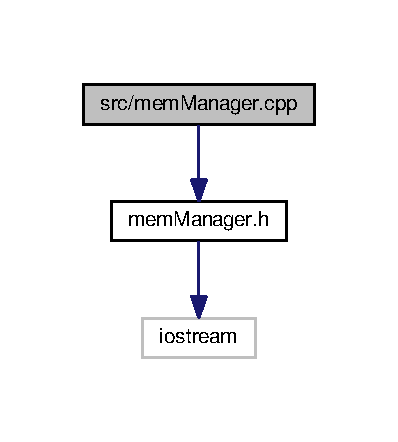
\includegraphics[width=191pt]{memManager_8cpp__incl}
\end{center}
\end{figure}
\subsection*{Funções}
\begin{DoxyCompactItemize}
\item 
{\footnotesize template$<$typename T $>$ }\\T $\ast$$\ast$ \hyperlink{memManager_8cpp_a82312208e9bea6d2b51e4ce4ee7436e5}{Aloc\+Matriz} (int n)
\begin{DoxyCompactList}\small\item\em Aloca os espaços da matriz dinamicamente. \end{DoxyCompactList}\item 
template int $\ast$$\ast$ {\bfseries Aloc\+Matriz$<$ int $>$} (int n)\hypertarget{memManager_8cpp_aa10215e720c4894474206659dfde58d6}{}\label{memManager_8cpp_aa10215e720c4894474206659dfde58d6}

\item 
{\footnotesize template$<$typename T $>$ }\\void \hyperlink{memManager_8cpp_a05e7a5a5adaabbe47ee044a33e137e4f}{delete\+Matriz} (T $\ast$$\ast$v, int n)
\begin{DoxyCompactList}\small\item\em Desaloca os espaços da matriz. \end{DoxyCompactList}\item 
template void {\bfseries delete\+Matriz$<$ int $>$} (int $\ast$$\ast$v, int n)\hypertarget{memManager_8cpp_ada2633d6c6343627a9d3f6eb9ebf08ff}{}\label{memManager_8cpp_ada2633d6c6343627a9d3f6eb9ebf08ff}

\end{DoxyCompactItemize}


\subsection{Descrição Detalhada}
Funções que alocam e desalocam espaços da memória utilizados pelas matrizes  Rodrigo Rocha Moriyama \href{mailto:rodrigo.oi@hotmail.com}{\tt rodrigo.\+oi@hotmail.\+com} \&\& Ariel de Oliveira Corrêa \href{mailto:ariel.oliveira01@gmail.com}{\tt ariel.\+oliveira01@gmail.\+com} 

\begin{DoxySince}{Desde}
28/04/2017  01/05/2017 
\end{DoxySince}


\subsection{Funções}
\index{mem\+Manager.\+cpp@{mem\+Manager.\+cpp}!Aloc\+Matriz@{Aloc\+Matriz}}
\index{Aloc\+Matriz@{Aloc\+Matriz}!mem\+Manager.\+cpp@{mem\+Manager.\+cpp}}
\subsubsection[{\texorpdfstring{Aloc\+Matriz(int n)}{AlocMatriz(int n)}}]{\setlength{\rightskip}{0pt plus 5cm}template$<$typename T $>$ T$\ast$$\ast$ Aloc\+Matriz (
\begin{DoxyParamCaption}
\item[{int}]{n}
\end{DoxyParamCaption}
)}\hypertarget{memManager_8cpp_a82312208e9bea6d2b51e4ce4ee7436e5}{}\label{memManager_8cpp_a82312208e9bea6d2b51e4ce4ee7436e5}


Aloca os espaços da matriz dinamicamente. 


\begin{DoxyParams}{Parâmetros}
{\em n} & Tamanho da Matriz Quadrada \\
\hline
\end{DoxyParams}
\begin{DoxyReturn}{Retorna}
Matriz Alocada 
\end{DoxyReturn}
\index{mem\+Manager.\+cpp@{mem\+Manager.\+cpp}!delete\+Matriz@{delete\+Matriz}}
\index{delete\+Matriz@{delete\+Matriz}!mem\+Manager.\+cpp@{mem\+Manager.\+cpp}}
\subsubsection[{\texorpdfstring{delete\+Matriz(\+T $\ast$$\ast$v, int n)}{deleteMatriz(T **v, int n)}}]{\setlength{\rightskip}{0pt plus 5cm}template$<$typename T $>$ void delete\+Matriz (
\begin{DoxyParamCaption}
\item[{T $\ast$$\ast$}]{v, }
\item[{int}]{n}
\end{DoxyParamCaption}
)}\hypertarget{memManager_8cpp_a05e7a5a5adaabbe47ee044a33e137e4f}{}\label{memManager_8cpp_a05e7a5a5adaabbe47ee044a33e137e4f}


Desaloca os espaços da matriz. 


\begin{DoxyParams}{Parâmetros}
{\em v} & Matriz de entrada \\
\hline
{\em n} & Tamanho da matriz \\
\hline
\end{DoxyParams}

%--- End generated contents ---

% Index
\backmatter
\newpage
\phantomsection
\clearemptydoublepage
\addcontentsline{toc}{chapter}{Índice}
\printindex

\end{document}
